\section{mo\-TS$<$ M $>$ Class Template Reference}
\label{classmo_t_s}\index{moTS@{moTS}}
Tabu Search (TS).  


{\tt \#include $<$mo\-TS.h$>$}

Inheritance diagram for mo\-TS$<$ M $>$::\begin{figure}[H]
\begin{center}
\leavevmode
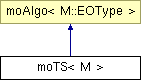
\includegraphics[height=5cm]{classmo_t_s}
\end{center}
\end{figure}
\subsection*{Public Member Functions}
\begin{CompactItemize}
\item 
{\bf mo\-TS} ({\bf mo\-Move\-Init}$<$ M $>$ \&\_\-move\_\-initializer, {\bf mo\-Next\-Move}$<$ M $>$ \&\_\-next\_\-move\_\-generator, {\bf mo\-Move\-Incr\-Eval}$<$ M $>$ \&\_\-incremental\_\-evaluation, {\bf mo\-Tabu\-List}$<$ M $>$ \&\_\-tabu\_\-list, {\bf mo\-Aspir\-Crit}$<$ M $>$ \&\_\-aspiration\_\-criterion, {\bf mo\-Sol\-Continue}$<$ {\bf EOT} $>$ \&\_\-continue, {\bf eo\-Eval\-Func}$<$ {\bf EOT} $>$ \&\_\-full\_\-evaluation)
\begin{CompactList}\small\item\em Constructor of a mo\-TS specifying all the boxes. \item\end{CompactList}\item 
{\bf mo\-TS} ({\bf mo\-Move\-Expl}$<$ M $>$ \&\_\-move\_\-explorer, {\bf mo\-Sol\-Continue}$<$ {\bf EOT} $>$ \&\_\-continue, {\bf eo\-Eval\-Func}$<$ {\bf EOT} $>$ \&\_\-full\_\-evaluation)
\begin{CompactList}\small\item\em Constructor with less parameters. \item\end{CompactList}\item 
bool {\bf operator()} ({\bf EOT} \&\_\-solution)
\begin{CompactList}\small\item\em Function which launchs the Tabu Search. \item\end{CompactList}\end{CompactItemize}
\subsection*{Private Types}
\begin{CompactItemize}
\item 
typedef M::EOType {\bf EOT}\label{classmo_t_s_y0}

\begin{CompactList}\small\item\em Alias for the type. \item\end{CompactList}\item 
typedef EOT::Fitness {\bf Fitness}\label{classmo_t_s_y1}

\begin{CompactList}\small\item\em Alias for the fitness. \item\end{CompactList}\end{CompactItemize}
\subsection*{Private Attributes}
\begin{CompactItemize}
\item 
{\bf mo\-Move\-Expl}$<$ M $>$ \& {\bf move\_\-explorer}\label{classmo_t_s_r0}

\begin{CompactList}\small\item\em Neighborhood explorer. \item\end{CompactList}\item 
{\bf mo\-Sol\-Continue}$<$ {\bf EOT} $>$ \& {\bf continu}\label{classmo_t_s_r1}

\begin{CompactList}\small\item\em Stop criterion. \item\end{CompactList}\item 
{\bf eo\-Eval\-Func}$<$ {\bf EOT} $>$ \& {\bf full\_\-evaluation}\label{classmo_t_s_r2}

\begin{CompactList}\small\item\em Full evaluation function. \item\end{CompactList}\end{CompactItemize}


\subsection{Detailed Description}
\subsubsection*{template$<$class M$>$ class mo\-TS$<$ M $>$}

Tabu Search (TS). 

Generic algorithm that describes a tabu search. 



Definition at line 50 of file mo\-TS.h.

\subsection{Constructor \& Destructor Documentation}
\index{moTS@{mo\-TS}!moTS@{moTS}}
\index{moTS@{moTS}!moTS@{mo\-TS}}
\subsubsection{\setlength{\rightskip}{0pt plus 5cm}template$<$class M$>$ {\bf mo\-TS}$<$ M $>$::{\bf mo\-TS} ({\bf mo\-Move\-Init}$<$ M $>$ \& {\em \_\-move\_\-initializer}, {\bf mo\-Next\-Move}$<$ M $>$ \& {\em \_\-next\_\-move\_\-generator}, {\bf mo\-Move\-Incr\-Eval}$<$ M $>$ \& {\em \_\-incremental\_\-evaluation}, {\bf mo\-Tabu\-List}$<$ M $>$ \& {\em \_\-tabu\_\-list}, {\bf mo\-Aspir\-Crit}$<$ M $>$ \& {\em \_\-aspiration\_\-criterion}, {\bf mo\-Sol\-Continue}$<$ {\bf EOT} $>$ \& {\em \_\-continue}, {\bf eo\-Eval\-Func}$<$ {\bf EOT} $>$ \& {\em \_\-full\_\-evaluation})\hspace{0.3cm}{\tt  [inline]}}\label{classmo_t_s_a0}


Constructor of a mo\-TS specifying all the boxes. 

In this constructor, a {\bf mo\-TSMove\-Loop\-Expl}{\rm (p.\,\pageref{classmo_t_s_move_loop_expl})} is instanciated.

\begin{Desc}
\item[Parameters:]
\begin{description}
\item[{\em \_\-move\_\-initializer}]The move initializer. \item[{\em \_\-next\_\-move\_\-generator}]The neighbourhood explorer. \item[{\em \_\-incremental\_\-evaluation}]The (generally) efficient evaluation. \item[{\em \_\-tabu\_\-list}]The tabu list. \item[{\em \_\-aspiration\_\-criterion}]An aspiration criterion. \item[{\em \_\-continue}]The stopping criterion. \item[{\em \_\-full\_\-evaluation}]A full evaluation function. \end{description}
\end{Desc}


Definition at line 72 of file mo\-TS.h.

References mo\-TS$<$ M $>$::continu, mo\-TS$<$ M $>$::full\_\-evaluation, and mo\-TS$<$ M $>$::move\_\-explorer.\index{moTS@{mo\-TS}!moTS@{moTS}}
\index{moTS@{moTS}!moTS@{mo\-TS}}
\subsubsection{\setlength{\rightskip}{0pt plus 5cm}template$<$class M$>$ {\bf mo\-TS}$<$ M $>$::{\bf mo\-TS} ({\bf mo\-Move\-Expl}$<$ M $>$ \& {\em \_\-move\_\-explorer}, {\bf mo\-Sol\-Continue}$<$ {\bf EOT} $>$ \& {\em \_\-continue}, {\bf eo\-Eval\-Func}$<$ {\bf EOT} $>$ \& {\em \_\-full\_\-evaluation})\hspace{0.3cm}{\tt  [inline]}}\label{classmo_t_s_a1}


Constructor with less parameters. 

The explorer is given in the parameters.

\begin{Desc}
\item[Parameters:]
\begin{description}
\item[{\em \_\-move\_\-explorer}]The explorer (generally different that a {\bf mo\-TSMove\-Loop\-Expl}{\rm (p.\,\pageref{classmo_t_s_move_loop_expl})}). \item[{\em \_\-continue}]The stopping criterion. \item[{\em \_\-full\_\-evaluation}]A full evaluation function. \end{description}
\end{Desc}


Definition at line 89 of file mo\-TS.h.

References mo\-TS$<$ M $>$::continu, mo\-TS$<$ M $>$::full\_\-evaluation, and mo\-TS$<$ M $>$::move\_\-explorer.

\subsection{Member Function Documentation}
\index{moTS@{mo\-TS}!operator()@{operator()}}
\index{operator()@{operator()}!moTS@{mo\-TS}}
\subsubsection{\setlength{\rightskip}{0pt plus 5cm}template$<$class M$>$ bool {\bf mo\-TS}$<$ M $>$::operator() ({\bf EOT} \& {\em \_\-solution})\hspace{0.3cm}{\tt  [inline]}}\label{classmo_t_s_a2}


Function which launchs the Tabu Search. 

Algorithm of the tabu search. As a {\bf mo\-SA}{\rm (p.\,\pageref{classmo_s_a})} or a {\bf mo\-HC}{\rm (p.\,\pageref{classmo_h_c})}, it can be used for HYBRIDATION in an evolutionary algorithm. For security a lock (pthread\_\-mutex\_\-t) is closed during the algorithm.

\begin{Desc}
\item[Parameters:]
\begin{description}
\item[{\em \_\-solution}]a solution to improve. \end{description}
\end{Desc}
\begin{Desc}
\item[Returns:]TRUE. \end{Desc}


Definition at line 102 of file mo\-TS.h.

References mo\-TS$<$ M $>$::continu, mo\-TS$<$ M $>$::EOT, mo\-TS$<$ M $>$::full\_\-evaluation, and mo\-TS$<$ M $>$::move\_\-explorer.

The documentation for this class was generated from the following file:\begin{CompactItemize}
\item 
mo\-TS.h\end{CompactItemize}
